%\vspace{0.3cm}
El objetivo principal de este capítulo es describir el diseño del framework propuesto para planificar tareas preemptive en sistemas embebidos heterogéneos. Se plantea la estructura del mismo junto con la descripción de su solución. 

Aunque se tomó como base el sistema embebido heterogéneo NVIDIA Jetson TX2, el diseño puede ser aplicado a cualquier dispositivo, siempre y cuando cumpla con la característica de tener memoria unificada, como la descrita en la sección \ref{sec:MemUni}.

\section{Descripción general del framework}

En la Figura \ref{fig:diagramabase} se muestra el diagrama a bloques que representa los elementos del framework propuesto. El primer bloque es el módulo de Puntos Preemptive, donde se plantea la propuesta para implementar el modo preemptive en las tareas, se contempla desde las directivas que se deben implementar hasta el manejo del contexto y sus variables. Justo después se describe un módulo en el que se engloban todos los aspectos del manejo de memoria entre el CPU y el GPU. Finalmente se tienen los módulos para la la planificación y la asignación de prioridades a cada tarea, las cuales son un complemento una de la otra para la correcta implementación de alguno de los algoritmos descritos en la sección \ref{sec:AlgoPlan}.

\vspace{0.3cm}

En los siguientes apartados de la tesis se analizarán y desglosarán cada uno de los módulos.
  \begin{figure}[ht]
      \centering
        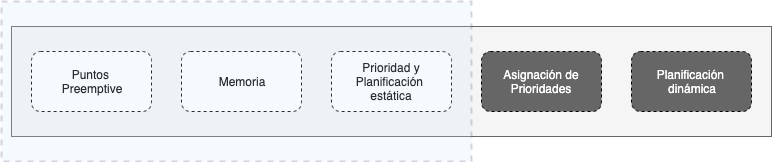
\includegraphics[scale=.8]{img/diagrama_framework}
        \caption{Diagrama del framework para la planificación de tareas preemptive en sistemas embebidos heterogéneos.}
        \label{fig:diagramabase}
    \end{figure}
  

  %Pero en el momento en el que se requiera tener un método de asignación de prioridades personalizado, es necesario tener un módulo que lo permita. Aunado a esto, si por alguna razón se solicita agregar tareas dinámicamente con el sistema en ejecución, se deben tener mecanismos para manejar cualquier interrupción o actualización de información del planificador. Ambos elementos son necesarios en un framework, pero sus componentes internos se dejarán para ser resueltos como trabajo futuro.
  
  \section{Puntos preemptive}\label{puntosPreemptive}

La mayoría de los trabajos relacionados en el estado del arte colocan puntos preemptive para formar fragmentos (chunks) de memoria.

Con esta solución se colocan puntos preemptive fijos dentro de las funciones kernel de la aplicación. Con esto se nos permite:

\begin{itemize}
\item Direccionar eventos.
\item Manejar las interrupciones de la tarea.
\item Modificar la granularidad de los subkernels.
\item Determinar las directivas para detener y restaurar una tarea.
\end{itemize}     
  
  \section{Memoria}
  
  En este apartado, 
  
  Como se mencionó en la sección \ref{puntosPreemptive}, la mayoría de los trabajos relacionados en el estado del arte colocan puntos preemptive para formar fragmentos (chunks) de memoria.
  
  La solución da prioridad a la creación de copias de memoria y transferencia entre GPU y CPU.
  
  La arquitectura del sistema permite el soporte de memoria unificada.
  
  No es necesario preocuparse por las transacciones de transferencia de datos.
  
  Disminución del consumo energético.
  
  Ahorro de recursos.
  
  \begin{figure}[ht]
      \centering
        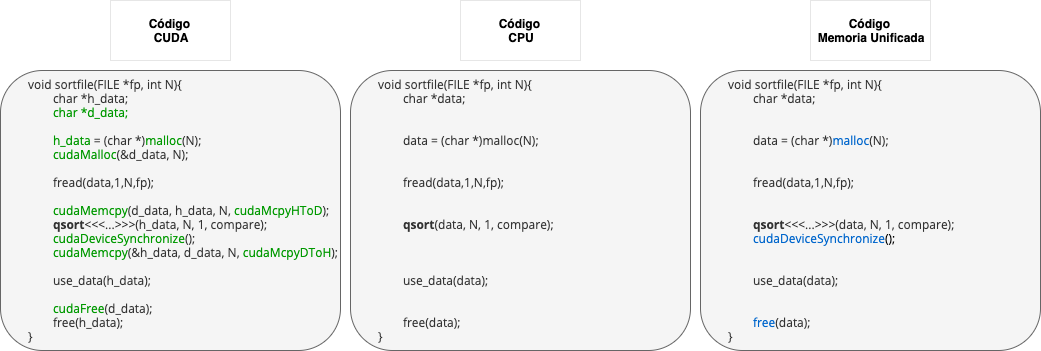
\includegraphics[scale=.50]{img/direcMem}
        \caption{Comparación de directivas para manejo de memoria.}
        \label{fig:direcMem}
    \end{figure}
  
\section{Planificación} 

\subsection{Planificación estática}

Sólo un artículo incluye soporte para la planificación con algoritmos en sistemas en tiempo real.

La prioridad es fija, ya que se asigna a partir de una cola FIFO.

Esta solución permite dar soporte para planificación con algoritmos de sistemas en tiempo real.

La prioridad puede ser estática o dinámica y está dada por el algoritmo de planificación.

\subsection{Planificación dinámica}
    	%Explicar por que es necesario, y por que no se aborda en este trabajo
\section{Asignación de prioridades }

\subsection{Asignación estática de prioridades }

\subsection{Asignación dinámica de prioridades }
    	%Explicar por que es necesario, y por que no se aborda en este trabajo
	La asignación de prioridades y la implementación de planificadores dinámicos de tareas de dejarán para trabajo futuro.
\section{Resumen}




